\section{Method}
\label{sec:methods}

\subsection{Computational details}
\label{subsec:DFT}

The electronic structure and, from it, the magnetic properties of the Fe-Co alloys were obtained using the fully self-consistent real-space linear muffin-tin orbital in the atomic sphere approximation (RS-LMTO-ASA) \cite{PhysRevB.44.13283,PhysRevB.46.14570}. In this first-principles scheme, the eigenvalue problem is solved directly in the real-space by employing Haydock recursion method \cite{Haydock1980} (for $LL$ recursion steps) together with Beer-Pettifor terminator \cite{Beer1984}, suitable for metallic systems. Here, the local spin density approximation (LSDA), with parametrization by von Barth and Hedin \cite{Barth1972}, was used for the exchange-correlation functional (XC). To evaluate the Gilbert damping in the torque-correlation method, the spin-orbit coupling (SOC) term, $\xi\hat{L}\cdot\hat{S}$, was included self-consistently at each variational step \cite{PhysRevB.69.104401}. 
The LMTO-ASA \cite{PhysRevB.12.3060} is a linear method that gives precise results around a given energy $E=E_{\nu}$, often chosen as the center of gravity of the $s$, $p$ and $d$ bands. Thus, as in the previous study \cite{PhysRevB.108.014433}, we consider an expression accurate to $(E-E_{\nu})^2$ starting from the orthogonal representation of LMTO-ASA -- given that nonlocal damping parameters are fine quantities. For all cases investigated, we considered $LL=31$, which produces reliable results for the damping of Fe-Co alloys when compared to available experimental and theoretical results in the literature \cite{PhysRevB.108.014433}.


In order to simulate alloys, we designed the following simulation protocol: we performed \textit{ab-initio} calculations on a virtual-crystal-approximation (VCA) medium of bcc FeCo alloys to account for the chemical disorder. In general, this approximation is well-known to be reasonable for systems where the energy bands behave more or less rigidly with changes in the alloy concentration -- which is exactly the case of FeCo, neighboring elements in the periodic table (for a more detailed discussion on the VCA for FeCo, see Appendix \ref{VCA}). Here, the medium matrix contains $\sim55000$ atoms. The Fe-Co alloys still maintain a body-centred-cubic (bcc) phase for the range of Co concentration from 0\% to 60\% \cite{schoen2016ultra} and the lattice parameter $a_0=2.87$\AA$\,$ was used for all values of $x$. Although the FeCo alloys present a slight variation of $\sim1\%$ in $a_0$ for $x\in[0\%,60\%]$ \cite{PhysRevB.93.224425,Ohnuma2002}, we keep $a_0$ fixed to concentrate on the effect coming solely from the chemical disorder. It also should be noticed that the composition of $x=60\%$ Co is at the edge of the transition to body-centred tetragonal (bct) phase \cite{andersson2006structure}, but for simplicity, we remain here in the bcc phase. As for the VCA approach we replace the nuclear charge ($Z$) and the number of valence electrons ($n_v$) by the alloy average based on the concentration, e.g., in the case of Fe$_{60}$Co$_{40}$ we consider $n_v=8.4$ and $Z=26.4$.

\begin{figure}[!ht] 
\centering
        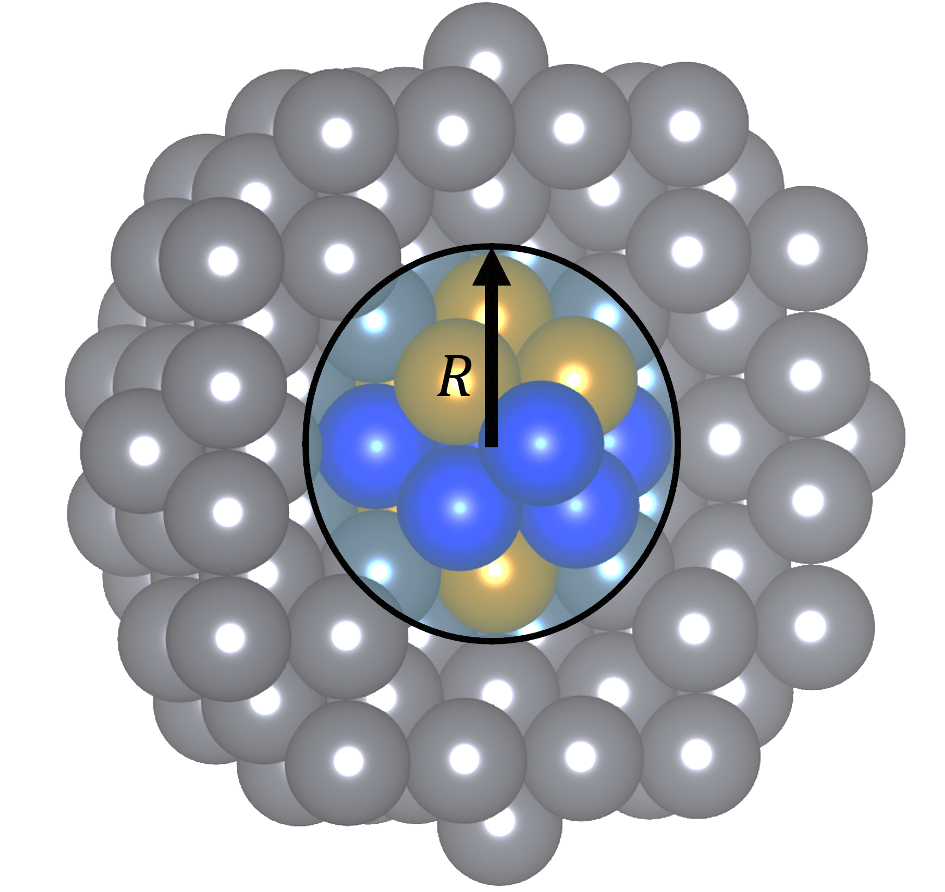
\includegraphics[width=0.7\columnwidth]{Fig1.png}
        \caption{(Color online) Schematic representation of the EC-VCA model in the bcc structure. The Fe and Co atoms are depicted by yellow and blue spheres, respectively, forming an explicit Fe$_{53}$Co$_{47}$ embedded cluster with radius $R$. In turn, the gray spheres symbolize the VCA medium mimicking the same alloy concentration, that extends significantly beyond the depicted limits (the full VCA matrix has $\sim55000$ atoms). Image produced with the VESTA software \cite{Momma2011}.} 
        \label{fig:ec-vca-representation} 
\end{figure}

After the self-consistent procedure on the pure VCA structure, $15$-atom clusters composed of different Fe and Co compositions as well as atomic arrangements were embedded into the center of the corresponding VCA medium as local impurities (see Figure \ref{fig:ec-vca-representation} for a schematic representation).

The impurity region was self-consistently treated while the potential parameters and Fermi energy of the pure VCA matrix host were kept fixed. This is a particularly suitable approach and certainly an improvement with respect to the simple VCA approximation, because the short-range disorder (which pure VCA neglects) is made explicit, while the more distant sites are replaced by the virtual atoms with long-range disorder properties. Naturally, this model tends to become more accurate whenever the radius $R$ of the explicit region increases, but with two main limitations: (\textit{i}) $R$ cannot be too close from the full medium matrix radius, to avoid any surface effects in real space; and (\textit{ii}) $R$ should be maximum to still be considered as a local perturbation, in which no appreciable change in the Fermi level of the crystalline host can be observed. As our intention here is to analyze the implications of very short range chemical disorder in the torque-correlation theory for the Gilbert damping (in its nonlocal formulation), the $15$-atom cluster ($R=a_0$) is a simple and useful model. From now on, this model will be referred to as \textit{embedded cluster VCA} (or, in short, EC-VCA).

From the electronic structure of this spatially disordered alloy, we determine both the onsite (for $i=j$) and the non-local (for $i\neq j$) contributions of the Gilbert damping $\alpha_{ij}$ from the following expression,

\begin{equation}\label{eq:damping-dft}
\begin{split}
\alpha_{ij}^{\mu\nu}=\frac{g}{m_i \pi}\int_{-\infty}^{\infty}\eta(\epsilon)\textnormal{Tr}\left(\hat{T}_{i}^{\mu}\hat{A}_{ij}(\epsilon_{+})(\hat{T}_{j}^{\nu})^{\dagger}\hat{A}_{ji}(\epsilon_{+})\right)d\epsilon,
\end{split}
\end{equation}

\noindent where $\epsilon_{+}=\epsilon+i\delta$ for some small positive value $\delta$ (in energy units), $\textnormal{Tr}$ denotes the trace, the hat notation (e.g., $\hat{A}$) is used for operators (or tensors), and $\hat{A}_{ij}(\epsilon_{+})=\frac{1}{2i}(\hat{G}_{ij}(\epsilon_{+})-\hat{G}_{ji}^{\dagger}(\epsilon_{+}))$ is the $ij$ block of the spectral function at the energy $\epsilon$. The imaginary part $\delta$ describes the electron band broadening and, thus, is related to the electron lifetime associated with the relaxation from an excited state to the ground state due to intrinsic scattering events. This involves electro-magnon and electron-phonon scattering as well as electron correlation. 

Typically $\delta$ serves as the input, as seen in Ref.~\cite{PhysRevLett.99.027204} or is calculated as a self-energy by dedicated methods, such as the alloy analogy model used in \cite{PhysRevLett.107.066603}. However, in our approach, it is determined from the terminated continued fractions in the Haydock recursion method. It has been shown previously that this procedure results in a good agreement of the Gilbert damping for several materials to experimental measurements \cite{PhysRevB.108.014433}. The term $\hat{T}^{\mu}_i=\left[\hat{\sigma}^{\mu}_i,\hat{\mathcal{H}}_{so}\right]$ is the so-called torque operator \cite{PhysRevMaterials.2.013801} at site $i$,  $\mu,\nu\in\{x,y,z\}$ represent the Cartesian coordinates, and $\eta(\epsilon)=-\frac{\partial f(\epsilon)}{\partial\epsilon}$ is the derivative of the Fermi-Dirac distribution $f(\epsilon)$ with respect to the energy $\epsilon$. In all our simulations, the electron temperature is here taken to be zero, so the energy integral is only performed at the Fermi level. The total magnetic moment at a site $i$, which is equal to the sum of orbital moment $m^{\textnormal{orb}}_{i}$ and spin moment $m^{\textnormal{spin}}_{i}$,  is represented by $m_{i}$. The $g$-factor is given by $g=2\left(1+\frac{m^{\textnormal{orb}}}{m^{\textnormal{spin}}}\right)$ and $\hat{\sigma}^{\mu}_i$ is the $\mu$-component of the Pauli matrices vector (at site $i$).

  Altogether, Eq. \ref{eq:damping-dft} implies that the non-local Gilbert damping is generally non-symmetric with respect to the $ij$ pairs, as also pointed out by Ref.~\cite{PhysRevB.109.094417}: 

\begin{equation}
\label{eq:symmetry-alphaij}
\alpha_{ij}^{\mu\nu} = \left(\frac{m_j^{\textnormal{spin}}}{m_i^{\textnormal{spin}}}\right)\alpha_{ji}^{\nu\mu},
\end{equation}

\noindent which should hold because of the trace properties applied to Eq. \ref{eq:damping-dft}. Naturally, Eq. \ref{eq:damping-dft} results in a $3\times3$ damping tensor $\alpha_{ij}^{\mu\nu}$. From having the spin quantization axis along the $\mathbf{z}$ ($[001]$) direction, we then can define a scalar damping value $\alpha_{ij}$ as the average $\alpha_{ij}=\frac{1}{2}(\alpha_{ij}^{xx}+\alpha_{ij}^{yy})$ (for a discussion about the validity of this definition in a chemical disorder environment, please see Section \ref{sec:off-diagonal-elements}). 

From the non-local Gilbert damping, we define the effective damping of atomic site $i$, $\alpha_i$, as

\begin{equation}\label{eq:damping_sum}
\begin{split}
\alpha_i =\sum_j \alpha_{ij}.
\end{split}
\end{equation}

In practice, $\alpha_i$ is the cumulative non-local damping summation inside a given cutoff radius $r_c$ from the reference ($i$-th) site: $\alpha_i=\sum_{r_{ij}\leq r_c}\alpha_{ij}$. Since $\alpha_{ij}$ is typically long-range and scales asymptotically (i.e., for large $r_{ij}$) as $1/r_{ij}^2$ \cite{PhysRevMaterials.2.013801,PhysRevB.108.014433,PhysRevB.109.094417}, we consider the sum not only over the 15 atoms in the embedded impurity cluster, but also into the VCA medium in the EC-VCA model. For $r_c=6a_0$, $\alpha_i$ is approximately converged, involving $1836$ neighboring atoms in the damping calculations plus the onsite term. 

Experiments often measure damping as a single parameter from ferromagnetic resonance (FMR) techniques~\cite{ma2017metrology,Schoen2016}, in which the magnetic moments are excited in a coherent mode ($\mathbf{q}=\mathbf{0}$). As demonstrated in Appendix \ref{sec:damping_formula}, the measured value (\textit{effective} damping, $\alpha^{\textnormal{eff}}$) can be related to the site-resolved effective damping $\alpha_i$ (Eq. \ref{eq:damping_sum}) as

\begin{equation}
\label{eq:total-damping}
\alpha^{\textnormal{eff}}=\frac{1}{\sum_i m_i}\sum_i \alpha_im_i,
\end{equation}

\noindent where the index $i$ runs over all atoms in the unit cell. For the general case, however, the relation is unfortunately not so straightforward; a correspondent $\alpha^{\textnormal{eff}}$ should be possible to be extracted by comparing how the magnetization behaves dynamically in the non-local damping environment and in a local, single-parameter $\alpha$ candidate. We note that previous investigations have engaged with the aspect of an \textit{averaged} $\alpha$ from element- or site-specific dampings, albeit  
without using the moments $m_i$ as weights (e.g., Ref. \cite{PhysRevB.95.214417}). For an alloy, several configurations can be constructed for a given concentration of elements. In that case, the average of \textit{all} obtained $\alpha^{\textnormal{eff}}$ values (for that concentration and chosen $\delta$) is the best theoretical estimation for a measured intrinsic $\alpha$. This quantitative analysis for all concentrations of the FeCo system is not the primary aim here, although we investigate the full scenario for an Fe-rich (Fe$_{87}$Co$_{13}$) alloy in \ref{subsec:local-effects-detailed}. Instead, our emphasis is directed towards the impact of the chemical environment on the $\alpha_i$, aiming for the report of \textit{locally hidden} features of that quantity.

\subsection{Atomistic spin dynamics with an explicit embedded cluster}

The generalized LLG equation \cite{PhysRevB.109.094417,PhysRevMaterials.2.013801,PhysRevB.108.014433,PhysRevB.73.184427}, which incorporates the nonlocal damping, is solved by using an implicit midpoint solver as implemented in the UppASD code \cite{UppASD}, with a time step of $dt=10^{-17}$ s; for more details on the solver and the spin Hamiltonian used see Ref. \cite{PhysRevB.108.014433}. In each simulation, a $40\times40\times40$ spin lattice with perfect bcc crystal symmetry is modelled with periodic boundary conditions. To isolate the effects of distinct magnetic interactions and damping parameters, all calculations start from the same random (noncollinear) spin state. The spin-spin exchange interactions and the nonlocal damping parameters are considered up to a cutoff radius of $r_c=6a_0$, in compliance with the convergence criteria established in Section \ref{subsec:DFT}. As in Ref. \cite{PhysRevB.108.014433}, the fluctuation-dissipation relation in the presence of nonlocal damping is considered up to the approximation $\alpha_{ij}^{\mu\nu}\rightarrow\frac{1}{3}\textnormal{Tr}(\hat{\alpha}_{ij})\delta_{ij}\delta_{\mu\nu}$, which is strictly reasonable in the low-temperature limit ($T\rightarrow0$), i.e., for vanishing stochastic fields. To break the rotational invariance of the Heisenberg exchange interaction term, a small cubic magnetic anisotropy was also added to the spin Hamiltonian. This term is characterized by an experimental constant $K_1$ of the order of $\sim3$ $\mu$eV/atom and easy axis $[100]$, approximately correspondent to the Fe$_{87}$Co$_{13}$ composition \cite{Pfeifer1980}. As all calculations include such anisotropy value, it thus does not contribute to the final differences observed.

When an embedded cluster is incorporated (i.e., beyond just VCA-type interactions), its 15-atom center coincides with the spin lattice center. Both $J_{ij}$ and $\alpha_{ij}$ parameters correspondent to each explicit Fe or Co sites (up to a distance of $6a_0$) are included in the Hamiltonian, considering the symmetry rules $J_{ij}=J_{ji}$ and the one defined in Eq. \ref{eq:symmetry-alphaij}. Of course, when short-range disorder is explicitly considered, the inversion symmetry is also broken, and Dzyaloshinskii-Moriya interactions can emerge as a consequence. As Fe and Co are elements with relatively weak spin-orbit coupling (which is also a cause of the $\sim10^{-3}$ intrinsic damping values), we choose to disregard that term in the Hamiltonian and concentrate on the effects of the inhomogeneous nonlocal damping field.


\subsection{Selected clusters and notation}
\label{subsec:clusters}

In our study, the embedded nano-clusters within the EC-VCA model are tailored to match the composition of the surrounding VCA medium. It is important to realize, however, that in a real sample this boundary is less sharp, and local configurations of solely Fe or Co (alloy clustering) are possible, albeit being less likely; this scenario is deliberately avoided here. Due to the vast number of possible configurations, our study specifically investigates a total of 64 unique configurations across all the compositions. The study is particularly concentrated on investigating the influence of neighboring Co atoms' positions on the effective damping of the central atom within each cluster configuration. For simplicity, the $\alpha_i$ refers to the effective damping of the central (reference) atom $i$ in each cluster in the following discussion. 

As we deal with several configurations, an appropriate notation system is imperative. Figure \ref{fig:cluster} illustrates the set of investigated Co-centered clusters in the Fe$_{53}$Co$_{47}$ composition, in which the horizontal axis depicts, from left to right, the embedded clusters with increasing number of Co atoms at the first neighboring shell (1st NN) of the reference atom $i$. Whenever possible, the notation will be exemplified with that particular composition, even though it is transferable to other Fe$_{100-x}$Co$_{x}$ alloys. Therefore, we adopt the following definitions and conventions:

\begin{itemize}
    \item$n$ denotes the number of Co atoms positioned at the first neighboring shell of the reference (central) site. For Fe$_{53}$Co$_{47}$, $n=\{0,1,\ldots,6\}$. However, it may exceed these values for Co-enhanced compositions (e.g., Fe$_{40}$Co$_{60}$);
    \item $d$ symbolizes the average interatomic distance among the Co atoms in the first neighboring shell (normalized by lattice constant $a_0$), calculated as 
    \begin{equation}
\label{eq:distance}
d=\frac{1}{n(n-1)}\sum_{ij}\frac{|\boldsymbol{r}_{ij}|}{a_0},
\end{equation}
    where  $\boldsymbol{r}_{ij}$ is the distance vector between Co atoms at sites $i$ and $j$; 
    \item $m=\{1,2,3\}$ groups the clusters based on the value of their averages distances $d$. Thus, $m=1$ and $m=3$ correspond to the clusters with the smallest and largest $d$, respectively, whereas $m=2$ identifies clusters that fall in between;
    \item C$n$ labels the cluster with $n$ Co atoms in the first neighboring shell, for a given alloy composition;
    \item C$n$-$m$ categorizes the cluster C$n$, identifying it with the proper Co average distance group $m$ (not used for the cases C0, C1, C7, and C8 by construction).
\end{itemize}
 
It should be noted that the possible number of average distances groups $m$ is larger than the 3 shown here. We have confined the number of clusters due to considerations of computational efficiency. Despite this constraint, the selected cases can adequately demonstrate the underlying physics. The investigated clusters can have the same 1st NN Co arrangement but a different 2nd NN environment in different compositions, attributed to the varying Co amounts. The total number of Co atoms and the maximum/minimum $n$ of each composition are shown in Table \ref{tab:cluster} in Appendix \ref{sec:Cluster_configuration}. 

 \begin{figure*}[!ht]
        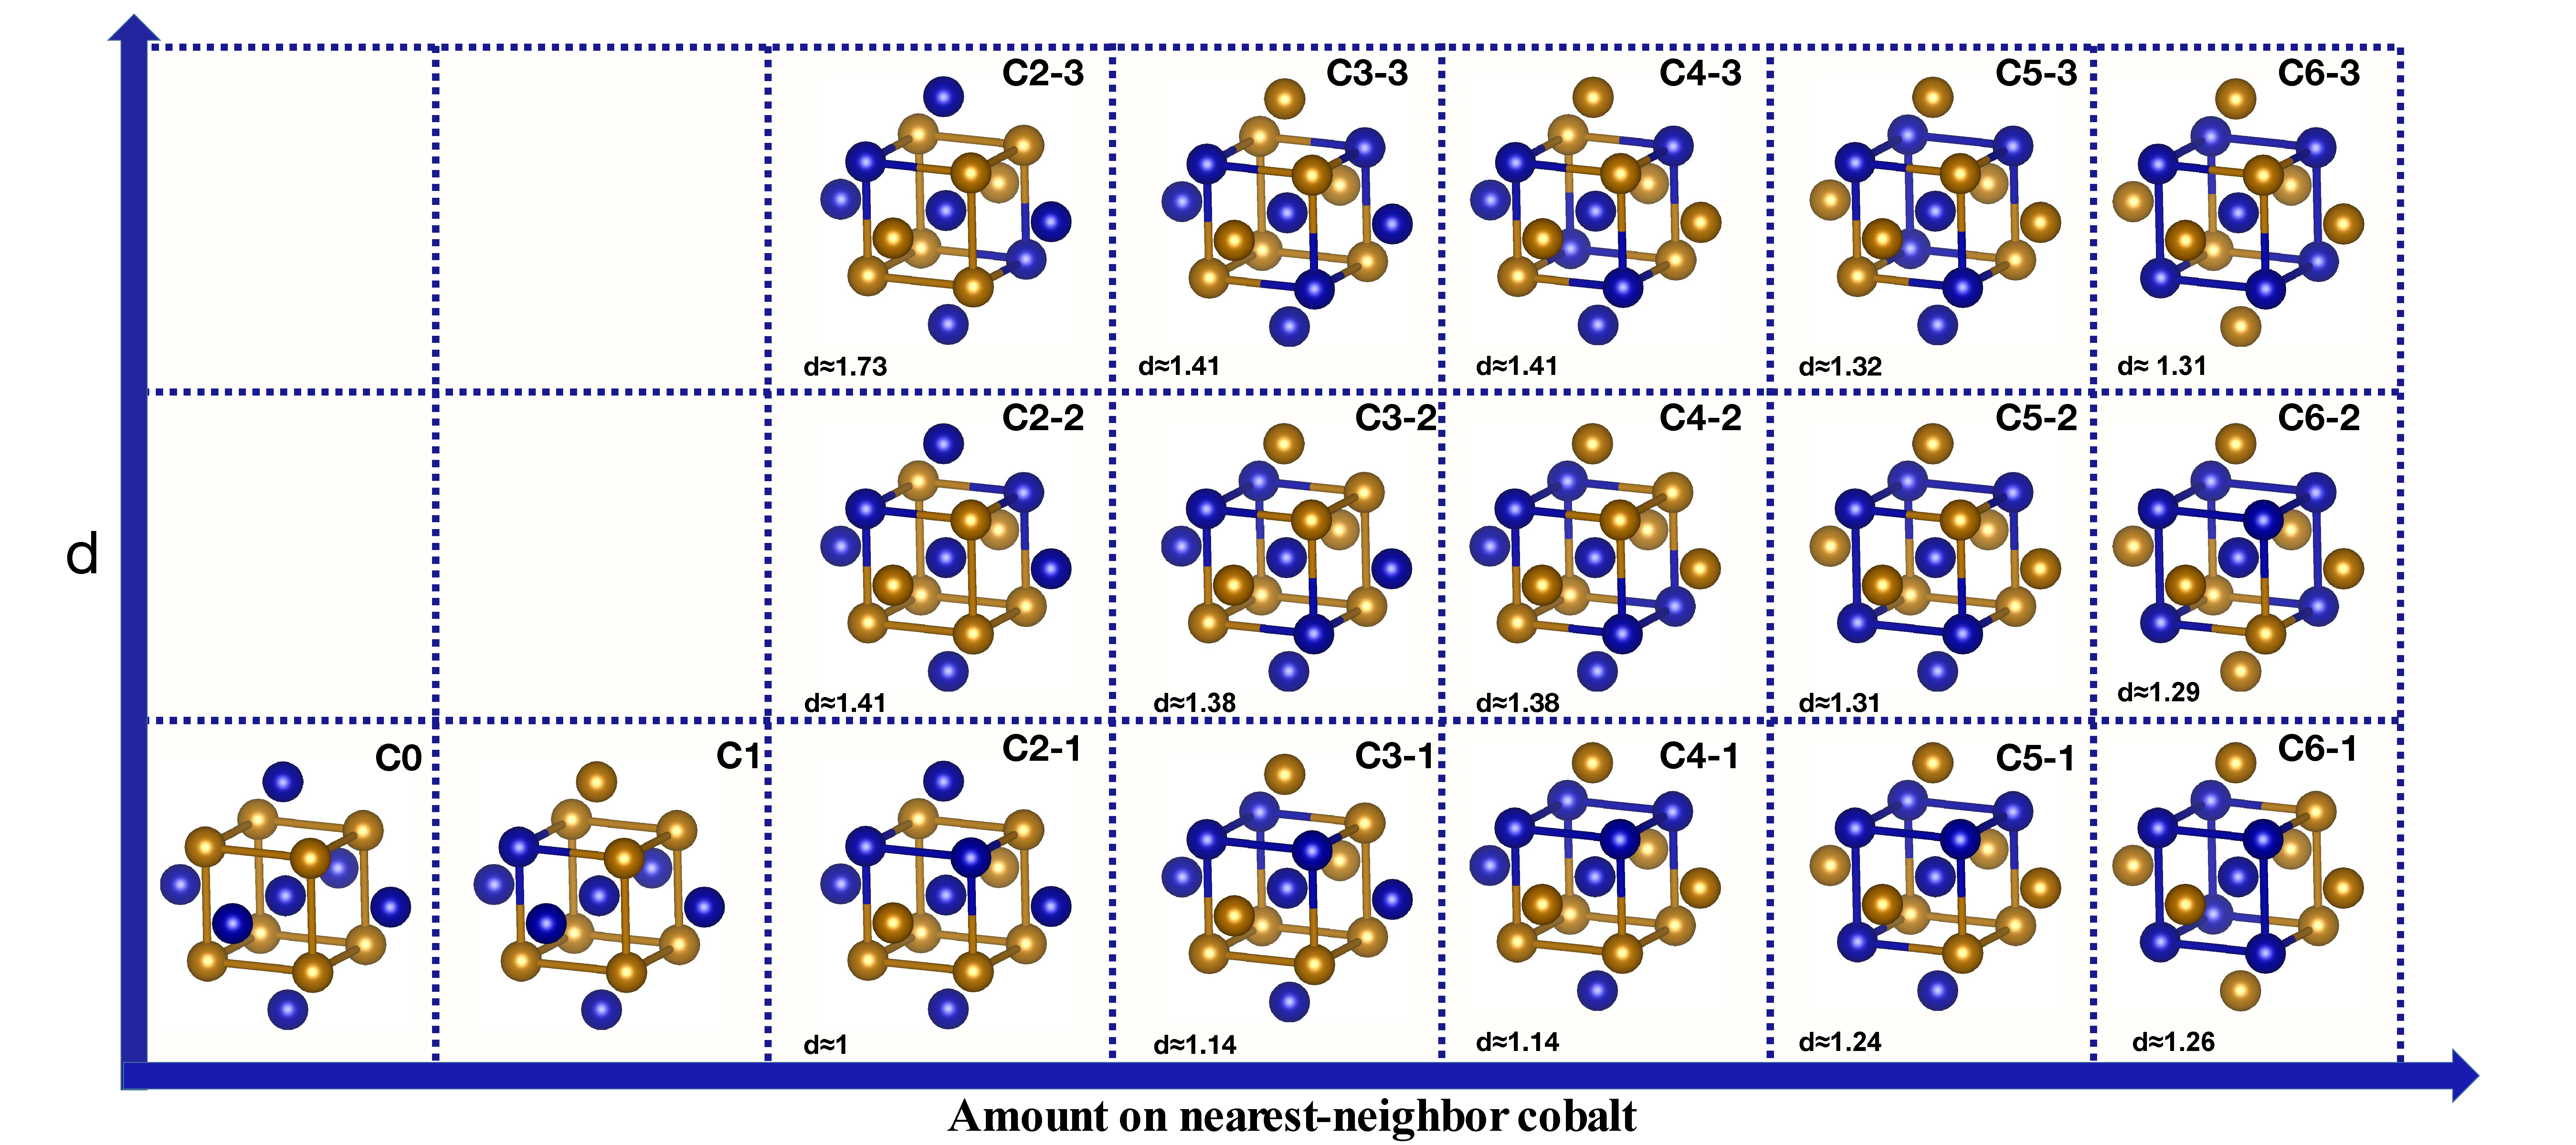
\includegraphics[width=2\columnwidth]{Fig2.pdf} 
        \caption{
        Schematic representation of some possible embedded Fe$_{53}$Co$_{47}$ clusters in the VCA medium. Within this composition, there are 8 Fe atoms (yellow spheres) and 7 Co atoms (blue spheres) in total.
        The horizontal line organizes, from left to right, the embedded clusters with increasing amount on nearest-neighbor cobalt $n$ (see text). Within each column, the clusters have the same $n$ but an increasing average Co interatomic distance $d$ defined in Eq. \ref{eq:distance}(in units of $a_0$)  from the bottom to the top side.}
        \label{fig:cluster} 
\end{figure*}
